\documentclass[aspectratio=169,10pt]{ctexbeamer}

\usetheme{default}
\usefonttheme{professionalfonts}
\setbeamertemplate{navigation symbols}{}
\setbeamertemplate{caption}[numbered]

\usepackage{amsmath,amssymb,bm}
\usepackage{booktabs}
\usepackage{array}
\usepackage{graphicx}
\usepackage{tikz}
\usepackage[most]{tcolorbox}
\usetikzlibrary{arrows.meta,positioning,calc,shapes.geometric}

\graphicspath{{../}}

\definecolor{DeepBlue}{HTML}{143A5A}
\definecolor{VBMBlue}{HTML}{1F77B4}
\definecolor{MSMOrange}{HTML}{F28E2B}
\definecolor{WarnRed}{HTML}{C44E52}
\definecolor{SoftGray}{HTML}{F4F6F8}
\definecolor{MidGray}{HTML}{6B7280}
\definecolor{SoftBlue}{HTML}{EAF3FB}
\definecolor{SoftYellow}{HTML}{FFF6D9}
\definecolor{SoftRed}{HTML}{FDEDEE}

\setbeamercolor{frametitle}{fg=DeepBlue,bg=white}
\setbeamerfont{frametitle}{series=\bfseries,size=\Large}
\setbeamercolor{normal text}{fg=black,bg=white}
\setbeamercolor{footline}{fg=MidGray,bg=white}
\setbeamertemplate{footline}{%
  \leavevmode%
  \hbox{%
    \begin{beamercolorbox}[wd=.72\paperwidth,ht=2.4ex,dp=1ex,leftskip=1.2em]{footline}%
      Huang \& Pimentel (2025) \quad | \quad Variance-based sensitivity analysis
    \end{beamercolorbox}%
    \begin{beamercolorbox}[wd=.28\paperwidth,ht=2.4ex,dp=1ex,rightskip=1.2em plus1fil]{footline}%
      \hfill \insertframenumber/\inserttotalframenumber
    \end{beamercolorbox}%
  }%
}

\tcbset{
  boxrule=0.7pt,
  arc=2.2mm,
  left=1.3mm,
  right=1.3mm,
  top=1mm,
  bottom=1mm,
  fonttitle=\bfseries
}

\newtcolorbox{bluebox}[1][]{
  colback=SoftBlue,
  colframe=VBMBlue,
  coltitle=white,
  #1
}
\newtcolorbox{orangebox}[1][]{
  colback=orange!7,
  colframe=MSMOrange,
  coltitle=white,
  #1
}
\newtcolorbox{yellowbox}[1][]{
  colback=SoftYellow,
  colframe=MSMOrange,
  coltitle=white,
  #1
}
\newtcolorbox{redbox}[1][]{
  colback=SoftRed,
  colframe=WarnRed,
  coltitle=white,
  #1
}
\newtcolorbox{graybox}[1][]{
  colback=SoftGray,
  colframe=MidGray,
  coltitle=white,
  #1
}

\newcommand{\keyword}[1]{\textcolor{DeepBlue}{\textbf{#1}}}
\newcommand{\vbm}[1]{\textcolor{VBMBlue}{\textbf{#1}}}
\newcommand{\msm}[1]{\textcolor{MSMOrange}{\textbf{#1}}}
\newcommand{\warn}[1]{\textcolor{WarnRed}{\textbf{#1}}}
\newcommand{\smallnote}[2][0.25em]{%
  \par\vspace{#1}%
  {\centering\scriptsize\color{MidGray}#2\par}%
}
\newcommand{\paperlink}{\href{https://doi.org/10.1093/biomet/asae040}{Huang \& Pimentel, \textit{Biometrika} 2025}}

\title{Variance-Based Sensitivity Analysis for Weighting Estimators}
\subtitle{From IPW weights to hidden-confounding stories}
\author[Group 1]{Group 1: Jialong Chen, Yining Shen, Kengyi Wang, Junyan Liu}
\institute{Biostatistics Final Project \textbar{} Group 1}
\date{\paperlink}

\begin{document}

% -------------------------------------------------------------------
\begin{frame}[plain]
  \vspace{0.65cm}
  {\Huge\bfseries\color{DeepBlue} Variance-based\\[0.08em] sensitivity analysis}

  \vspace{0.45cm}
  {\Large From IPW weights to hidden-confounding stories}

  \vspace{0.75cm}
  \begin{columns}[T,totalwidth=\textwidth]
    \begin{column}{0.30\textwidth}
      \begin{orangebox}
        \centering
        {\huge $L_\infty$}\\[0.35em]
        \textbf{worst individual}
      \end{orangebox}
    \end{column}
    \begin{column}{0.30\textwidth}
      \begin{bluebox}
        \centering
        {\huge $L_2/R^2$}\\[0.35em]
        \textbf{overall imbalance}
      \end{bluebox}
    \end{column}
    \begin{column}{0.30\textwidth}
      \begin{yellowbox}
        \centering
        {\huge $L_1$/TV}\\[0.35em]
        \textbf{mass-moving budget}
      \end{yellowbox}
    \end{column}
  \end{columns}

  \vfill
  \begin{flushright}
    \small
    \paperlink\\
    Group 1
  \end{flushright}
\end{frame}

% -------------------------------------------------------------------
\begin{frame}{Start with the causal question and notation}
  \begin{columns}[T,totalwidth=\textwidth]
    \begin{column}{0.45\textwidth}
      \begin{bluebox}[title=NHANES application]
        \begin{itemize}
          \item \keyword{$Z$}: high fish/shellfish consumption
          \item \keyword{$Y$}: $\log_2$(total blood mercury)
          \item \keyword{$X$}: observed covariates
          \item \keyword{$U$}: hidden confounder
        \end{itemize}
      \end{bluebox}
      \vspace{0.35cm}
      \begin{redbox}
        \centering
        Fish consumption is not randomized: diet, income, education, race, and health awareness may all matter.
      \end{redbox}
    \end{column}
    \begin{column}{0.51\textwidth}
      \begin{graybox}[title=Target estimand]
        \[
          \tau = E\{Y(1)-Y(0)\mid Z=1\}
        \]
        \[
          = E\{Y(1)\mid Z=1\} - E\{Y(0)\mid Z=1\}
        \]
      \end{graybox}
      \vspace{0.35cm}
      \begin{yellowbox}
        \centering
        The missing object is the treated group's counterfactual control outcome:
        \[
          E\{Y(0)\mid Z=1\}.
        \]
      \end{yellowbox}
    \end{column}
  \end{columns}
\end{frame}

% -------------------------------------------------------------------
\begin{frame}{IPW uses controls to approximate the missing counterfactual}
  \begin{columns}[T,totalwidth=\textwidth]
    \begin{column}{0.48\textwidth}
      \begin{bluebox}[title=Observable ATT weighting estimator]
        \small
        \[
          \tau(w)=
          E(Y\mid Z=1)
          -
          E\{w(X)Y\mid Z=0\}
        \]
        \[
          w(X)=\frac{f_{X\mid Z=1}(X)}{f_{X\mid Z=0}(X)}
        \]
      \end{bluebox}
      \vspace{0.25cm}
      \begin{graybox}
        \centering
        Larger control weight = ``this control looks more like the treated group.''
      \end{graybox}
    \end{column}
    \begin{column}{0.48\textwidth}
      \centering
      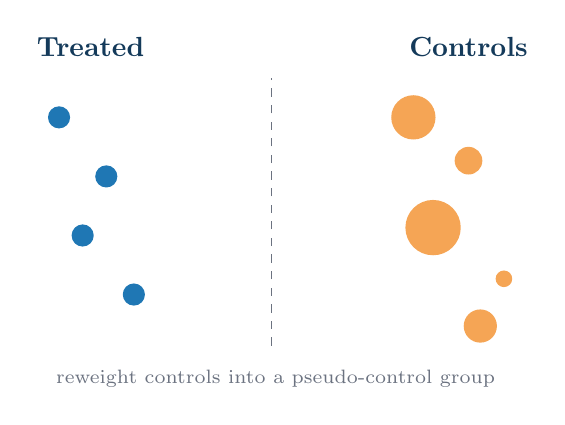
\begin{tikzpicture}[x=1cm,y=1cm]
        \node[font=\bfseries,color=DeepBlue] at (0,4.0) {Treated};
        \node[font=\bfseries,color=DeepBlue] at (4.8,4.0) {Controls};
        \foreach \x/\y in {-0.4/3.1,0.2/2.35,-0.1/1.6,0.55/0.85} {
          \fill[VBMBlue] (\x,\y) circle (4pt);
        }
        \foreach \x/\y/\s in {4.1/3.1/8,4.8/2.55/5,4.35/1.7/10,5.25/1.05/3,4.95/0.45/6} {
          \fill[MSMOrange!80] (\x,\y) circle (\s pt);
        }
        \draw[dashed,color=MidGray] (2.3,0.2) -- (2.3,3.6);
        \node[font=\scriptsize,color=MidGray] at (2.35,-0.22) {reweight controls into a pseudo-control group};
      \end{tikzpicture}
    \end{column}
  \end{columns}
\end{frame}

% -------------------------------------------------------------------
\begin{frame}{Hidden confounding means the ideal weights are different}
  \begin{columns}[T,totalwidth=\textwidth]
    \begin{column}{0.48\textwidth}
      \begin{bluebox}[title=Observable weights]
        \[
          w(X)=
          \frac{\Pr(Z=0)\Pr(Z=1\mid X)}
              {\Pr(Z=1)\Pr(Z=0\mid X)}
        \]
      \end{bluebox}
      \vspace{0.3cm}
      \begin{redbox}[title=Ideal weights]
        \[
          w^*(X,U)=
          \frac{\Pr(Z=0)\Pr(Z=1\mid X,U)}
              {\Pr(Z=1)\Pr(Z=0\mid X,U)}
        \]
      \end{redbox}
    \end{column}
    \begin{column}{0.48\textwidth}
      \begin{yellowbox}[title=Bias is a weight problem]
        \[
          \mathrm{Bias}=\tau(w)-\tau(w^*)
        \]
        \[
          \lambda=\frac{w^*}{w}
        \]
      \end{yellowbox}
      \vspace{0.25cm}
      \begin{graybox}
        Sensitivity analysis does not identify $U$. It asks how much $\lambda$ could move before the conclusion breaks.
      \end{graybox}
    \end{column}
  \end{columns}
\end{frame}

% -------------------------------------------------------------------
\begin{frame}{Sensitivity analysis is a three-step calculation}
  \vspace{0.15cm}
  \begin{center}
    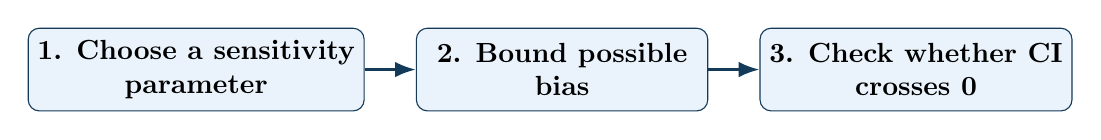
\begin{tikzpicture}[node distance=0.65cm,>=Latex]
      \node[draw=DeepBlue,fill=SoftBlue,rounded corners,align=center,minimum width=3.7cm,minimum height=1.05cm,font=\bfseries] (a)
        {1. Choose a sensitivity\\parameter};
      \node[draw=DeepBlue,fill=SoftBlue,rounded corners,align=center,minimum width=3.7cm,minimum height=1.05cm,font=\bfseries,right=of a] (b)
        {2. Bound possible\\bias};
      \node[draw=DeepBlue,fill=SoftBlue,rounded corners,align=center,minimum width=3.7cm,minimum height=1.05cm,font=\bfseries,right=of b] (c)
        {3. Check whether CI\\crosses 0};
      \draw[->,line width=1pt,color=DeepBlue] (a) -- (b);
      \draw[->,line width=1pt,color=DeepBlue] (b) -- (c);
    \end{tikzpicture}
  \end{center}

  \vspace{0.55cm}
  \begin{columns}[T,totalwidth=\textwidth]
    \begin{column}{0.31\textwidth}
      \begin{orangebox}
        \centering
        $\Gamma$ in MSM\\
        \small max odds-ratio multiplier
      \end{orangebox}
    \end{column}
    \begin{column}{0.31\textwidth}
      \begin{bluebox}
        \centering
        $R^2$ in VBM\\
        \small residual weight variance
      \end{bluebox}
    \end{column}
    \begin{column}{0.31\textwidth}
      \begin{yellowbox}
        \centering
        $T$ in RGM\\
        \small total-variation budget
      \end{yellowbox}
    \end{column}
  \end{columns}
\end{frame}

% -------------------------------------------------------------------
\begin{frame}{Baseline: MSM uses an $L_\infty$ constraint}
  \begin{columns}[T,totalwidth=\textwidth]
    \begin{column}{0.48\textwidth}
      \begin{orangebox}[title=Marginal sensitivity model]
        \[
          \Gamma^{-1}\leq \frac{w^*(X,U)}{w(X)} \leq \Gamma
        \]
        \[
          \lambda=\frac{w^*}{w},
          \qquad
          \|\lambda\|_\infty \leq \Gamma
        \]
      \end{orangebox}
      \vspace{0.3cm}
      \begin{graybox}[title=Definition]
        \small
        $\Gamma$ is the largest allowed individual weight-ratio distortion.
        MSM protects against the worst allowed unit-level deviation.
      \end{graybox}
    \end{column}
    \begin{column}{0.48\textwidth}
      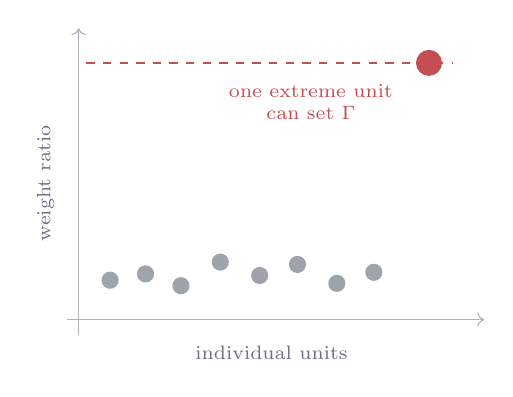
\begin{tikzpicture}[x=1cm,y=1cm]
        \draw[->, color=MidGray!55] (0.25,0.52) -- (5.55,0.52);
        \draw[->, color=MidGray!55] (0.40,0.32) -- (0.40,4.22);

        \foreach \x/\y in {0.80/1.02,1.25/1.10,1.70/0.95,2.20/1.25,2.70/1.08,3.18/1.22,3.68/0.98,4.15/1.12}
          \fill[MidGray!65] (\x,\y) circle (3.1pt);

        \fill[WarnRed] (4.85,3.78) circle (4.7pt);
        \draw[dashed, WarnRed, line width=0.75pt] (0.50,3.78) -- (5.15,3.78);

        \node[align=center, font=\scriptsize, color=WarnRed, text width=2.8cm] at (3.35,3.28)
          {one extreme unit\\can set $\Gamma$};
        \node[font=\scriptsize, color=MidGray] at (2.85,0.10) {individual units};
        \node[rotate=90, font=\scriptsize, color=MidGray] at (-0.02,2.25) {weight ratio};
      \end{tikzpicture}

      \vspace{0.12cm}
      \begin{redbox}[title=Cost]
        \small A rare extreme ratio can dominate the sensitivity parameter.
      \end{redbox}
    \end{column}
  \end{columns}
\end{frame}

% -------------------------------------------------------------------
\begin{frame}{Why the paper looks beyond $L_\infty$}
  \begin{columns}[T,totalwidth=\textwidth]
    \begin{column}{0.48\textwidth}
      \begin{redbox}[title=Problem 1: ratio-driven]
        \[
          \widehat{\Gamma}
          =
          \max_i
          \left\{
          \frac{w_i^*}{w_i},
          \frac{w_i}{w_i^*}
          \right\}
        \]
        \small With more samples, a rare extreme ratio becomes more likely.
      \end{redbox}
    \end{column}
    \begin{column}{0.48\textwidth}
      \begin{redbox}[title=Problem 2: sample-bounded]
        \[
          \bar Y_{0,q}
          \in
          [\min_{Z_i=0}Y_i,\ \max_{Z_i=0}Y_i]
        \]
        \small Reweighting observed controls cannot create counterfactual outcomes outside the observed control range.
      \end{redbox}
    \end{column}
  \end{columns}
  \vspace{0.55cm}
  \begin{yellowbox}
    \centering
    The paper's move: measure hidden confounding by \textbf{distribution-level weight variance}, not the worst individual ratio.
  \end{yellowbox}
\end{frame}

% -------------------------------------------------------------------
\begin{frame}{VBM measures unexplained variance in the ideal weights}
  \begin{columns}[T,totalwidth=\textwidth]
    \begin{column}{0.56\textwidth}
      \begin{bluebox}[title=Variance-based sensitivity parameter]
        \[
          R^2
          =
          1-
          \frac{\mathrm{Var}\{w(X)\mid Z=0\}}
              {\mathrm{Var}\{w^*(X,U)\mid Z=0\}}
        \]
      \end{bluebox}
      \vspace{0.25cm}
      \begin{graybox}
        \begin{itemize}
          \item $R^2=0$: hidden $U$ adds no residual weight imbalance.
          \item $R^2\to1$: ideal-weight variance is mostly due to hidden $U$.
        \end{itemize}
      \end{graybox}
    \end{column}
    \begin{column}{0.40\textwidth}
      \begin{yellowbox}[title=Sensitivity set]
        \small
        Possible ideal weights satisfy:
        \[
          1\le
          \frac{\mathrm{Var}(w^*)}{\mathrm{Var}(w)}
          \le
          \frac{1}{1-R^2}
        \]
        Larger $R^2$ allows more hidden weight variance.
      \end{yellowbox}
    \end{column}
  \end{columns}
\end{frame}

% -------------------------------------------------------------------
\begin{frame}{Theorem 1 turns $R^2$ into a bias envelope}
  \begin{bluebox}[title=Closed-form bound]
    \[
      B(R^2)=
      \sqrt{1-\rho_{wY}^2}\,
      \sqrt{
        \frac{R^2}{1-R^2}\,
        \mathrm{Var}(Y\mid Z=0)\mathrm{Var}(w\mid Z=0)
      }
    \]
    \[
      \tau(w^*)\in
      [\,\tau(w)-B(R^2),\ \tau(w)+B(R^2)\,],
      \qquad
      \rho_{wY}=\mathrm{cor}(w,Y\mid Z=0).
    \]
  \end{bluebox}
  \vspace{0.25cm}
  \begin{columns}[T,totalwidth=\textwidth]
    \begin{column}{0.48\textwidth}
      \begin{graybox}[title=Proof intuition]
        \[
          \mathrm{Bias}\approx
          \mathrm{Cov}(w^*-w,\ Y\mid Z=0)
        \]
        Cauchy--Schwarz turns covariance into a variance bound.
      \end{graybox}
    \end{column}
    \begin{column}{0.48\textwidth}
      \begin{yellowbox}[title=Inference]
        Percentile bootstrap adds sampling uncertainty around the bound.
      \end{yellowbox}
    \end{column}
  \end{columns}
\end{frame}

% -------------------------------------------------------------------
\begin{frame}{Theorem 3 reveals the geometry: $L_\infty$ vs weighted $L_2$}
  \begin{columns}[T,totalwidth=\textwidth]
    \begin{column}{0.32\textwidth}
      \begin{orangebox}
        \centering
        {\huge $L_\infty$}\\[0.3em]
        \textbf{MSM}\\[0.25em]
        \[
          \|\lambda\|_\infty\le \Gamma
        \]
        \small worst individual ratio
      \end{orangebox}
    \end{column}
    \begin{column}{0.32\textwidth}
      \begin{bluebox}
        \centering
        {\huge $L_2/R^2$}\\[0.3em]
        \textbf{VBM}\\[0.25em]
        \[
          \|\lambda\|_{2,w}^2
          =
          E_w(\lambda^2)
        \]
        \small average squared perturbation
      \end{bluebox}
    \end{column}
    \begin{column}{0.32\textwidth}
      \begin{yellowbox}
        \centering
        {\huge $L_1$/TV}\\[0.3em]
        \textbf{RGM extension}\\[0.25em]
        \[
          T=\frac12 E(|w^*-w|\mid Z=0)
        \]
        \small total mass shift
      \end{yellowbox}
    \end{column}
  \end{columns}
  \vspace{0.15cm}
  \begin{graybox}
    \small
    \textbf{Theorem 3:} the $R^2$ sensitivity set is equivalently a weighted-$L_2$ constraint on
    $\lambda=w^*/w$:
    \[
      \|\lambda\|_{2,w}\le \sqrt{k/(1-R^2)},
      \quad
      k=1-\frac{R^2}{E(w^2\mid Z=0)}.
    \]
    This is why the paper's comparison with MSM is really $L_2$ vs. $L_\infty$.
  \end{graybox}
\end{frame}

% -------------------------------------------------------------------
\begin{frame}{Data review: same NHANES sample, packaged in R}
  \begin{columns}[T,totalwidth=\textwidth]
    \begin{column}{0.39\textwidth}
      \begin{bluebox}
        \centering
        {\Huge 1107}\\
        total sample size
      \end{bluebox}
      \vspace{0.25cm}
      \begin{bluebox}
        \centering
        {\Huge 234}\\
        treated
      \end{bluebox}
      \vspace{0.25cm}
      \begin{bluebox}
        \centering
        {\Huge 873}\\
        controls
      \end{bluebox}
    \end{column}
    \begin{column}{0.55\textwidth}
      \begin{graybox}[title=Data source]
        \begin{itemize}
          \item Packaged file: \texttt{nhanes.fish.rda}
          \item Survey source: CDC/NCHS NHANES 2013--2014
          \item Outcome: $\log_2$(total blood mercury)
          \item Treatment: high fish/shellfish consumption
        \end{itemize}
      \end{graybox}
      \vspace{0.35cm}
      \begin{yellowbox}
        \centering
        This is not a second dataset; it is the paper's NHANES fish-mercury analysis sample.
      \end{yellowbox}
    \end{column}
  \end{columns}
\end{frame}

% -------------------------------------------------------------------
\begin{frame}{Our replication closely matches the paper}
  \vspace{0.15cm}
  \begin{columns}[T,totalwidth=\textwidth]
    \begin{column}{0.31\textwidth}
      \begin{bluebox}
        \centering
        \textbf{Unweighted ATT}\\[0.45em]
        {\Huge 2.368}\\[0.35em]
        \small paper: 2.37
      \end{bluebox}
    \end{column}
    \begin{column}{0.31\textwidth}
      \begin{bluebox}
        \centering
        \textbf{IPW ATT}\\[0.45em]
        {\Huge 2.093}\\[0.35em]
        \small paper: 2.14
      \end{bluebox}
    \end{column}
    \begin{column}{0.31\textwidth}
      \begin{bluebox}
        \centering
        \textbf{VBM $R^{2*}$}\\[0.45em]
        {\Huge 0.519}\\[0.35em]
        \small paper: 0.52
      \end{bluebox}
    \end{column}
  \end{columns}
\end{frame}

% -------------------------------------------------------------------
\begin{frame}{VBM sensitivity profile crosses the null near $R^2=0.52$}
  \begin{columns}[T,totalwidth=\textwidth]
    \begin{column}{0.70\textwidth}
      \includegraphics[width=\linewidth,height=0.68\textheight,keepaspectratio]{version10.1/output/figures_enhanced/figure1_vbm_paper_style.png}
    \end{column}
    \begin{column}{0.27\textwidth}
      \begin{graybox}[title=Read the figure]
        \small
        \begin{itemize}
          \item blue intervals: 95\% bootstrap CI
          \item horizontal dashed line: null effect
          \item vertical dotted line: $R^{2*}\approx0.52$
        \end{itemize}
      \end{graybox}
      \vspace{0.25cm}
      \begin{bluebox}
        \centering
        \small The conclusion loses significance only when hidden $U$ explains roughly half of ideal-weight variance.
      \end{bluebox}
    \end{column}
  \end{columns}
\end{frame}

% -------------------------------------------------------------------
\begin{frame}{Benchmarking makes $R^2$ interpretable}
  \begin{columns}[T,totalwidth=\textwidth]
    \begin{column}{0.69\textwidth}
      \includegraphics[width=\linewidth,height=0.68\textheight,keepaspectratio]{version10.1/output/figures_enhanced/figure3_benchmark_paper_style.png}
    \end{column}
    \begin{column}{0.28\textwidth}
      \begin{bluebox}[title=VBM benchmarks]
        \small
        Race: $R^2=0.240$\\
        Education: $R^2=0.210$\\
        Income: $R^2=0.172$\\[0.25em]
        \textbf{Threshold: $R^{2*}=0.519$}
      \end{bluebox}
      \vspace{0.25cm}
      \begin{yellowbox}
        \small Known covariate-level hidden confounding is not enough to overturn the NHANES conclusion under VBM.
      \end{yellowbox}
    \end{column}
  \end{columns}
\end{frame}

% -------------------------------------------------------------------
\begin{frame}{$L_1$/TV extension: RGM asks how much mass can move}
  \begin{columns}[T,totalwidth=\textwidth]
    \begin{column}{0.58\textwidth}
      \includegraphics[width=\linewidth,height=0.68\textheight,keepaspectratio]{version10.1/output/version10_extension_results/04_rgm_vbm_msm/figures_enhanced/enhanced_rgm_sharp_curve.png}
    \end{column}
    \begin{column}{0.38\textwidth}
      \begin{yellowbox}[title=RGM sharp model]
        \[
          T=\frac12\sum_i |q_i-p_i|
        \]
        \small $T$ is a total-variation budget: how much control-weight mass hidden confounding may move.
      \end{yellowbox}
      \vspace{0.25cm}
      \begin{bluebox}[title=Existing result]
        \small
        Sharp RGM interval crosses 0 around
        \[
          T^*\approx0.393.
        \]
        It directly models sparse/local bias.
      \end{bluebox}
    \end{column}
  \end{columns}
\end{frame}

% -------------------------------------------------------------------
\begin{frame}{Hidden-strength extension: stress-test detection power}
  \begin{columns}[T,totalwidth=\textwidth]
    \begin{column}{0.70\textwidth}
      \includegraphics[width=\linewidth,height=0.68\textheight,keepaspectratio]{version10.1/output/version10_extension_results/01_hidden_strength_vbm_msm/figures_enhanced/synthetic_vbm_msm_detection_power_by_strength.png}
    \end{column}
    \begin{column}{0.27\textwidth}
      \begin{graybox}[title=Read the extension]
        \small
        \begin{itemize}
          \item Hidden strength increases from H0 to H5.
          \item MSM reaches the null earlier.
          \item VBM is more conservative until severe hidden confounding.
        \end{itemize}
      \end{graybox}
      \vspace{0.25cm}
      \begin{bluebox}
        \small\raggedright
        \textbf{Lesson:} different norms see different hidden-bias shapes.
      \end{bluebox}
    \end{column}
  \end{columns}
\end{frame}

% -------------------------------------------------------------------
\begin{frame}{Takeaways and limitations}
  \vspace{0.2cm}
  \begin{enumerate}
    \item \keyword{IPW is a weighting solution to a missing-counterfactual problem.}
    \vspace{0.35em}
    \item \vbm{VBM replaces worst individual ratio with residual weight variance.}
    \vspace{0.35em}
    \item \msm{$L_\infty$}, \vbm{$L_2/R^2$}, and \keyword{$L_1$/TV} answer different hidden-confounding stories.
  \end{enumerate}

  \vspace{0.5cm}
  \begin{redbox}[title=Limitations worth saying out loud]
    \small
    \begin{itemize}
      \item VBM is not uniformly tighter than MSM.
      \item Sparse/local hidden bias may be more natural under $L_1$/TV.
      \item Bootstrap validity and $R^2$ calibration depend on propensity modeling and stable $\mathrm{Var}(w)$.
    \end{itemize}
  \end{redbox}
\end{frame}

% -------------------------------------------------------------------
\begin{frame}[plain]
  \vspace{1.2cm}
  \begin{center}
    {\Huge\bfseries\color{DeepBlue} Thank you!}\\[0.55cm]

    \vspace{0.8cm}
    \begin{bluebox}[width=0.8\textwidth]
      \centering
      \large Sensitivity analysis should make hidden assumptions visible.
    \end{bluebox}

    \vspace{0.45cm}
    {\small\color{MidGray}
    GitHub repository: \texttt{https://github.com/Syn-fdu/VBM-implementation}}

    \vspace{0.55cm}
    {\small\color{MidGray}
    Group 1}
  \end{center}
\end{frame}

\end{document}
